When looking at both the TAPE paper\cite{tape} and the Unirep paper\cite{unirep}, they have some conflicting information regarding the Spearman correlation they achieve when predicting stability scores. The Unirep paper says that they get a Spearman correlation score of $0.59$, but we could not find the dataset they used to get this on. We used the TAPE dataset, in whose paper they say that Unirep scores a significantly better $0.73$. With our best model's score of $0.627$ we would consider this a pretty good result. We also generated a TSNE plot with the output of this model, which can be compared to a similar Unirep model in Figure ~\ref{fig:unirep_comp}

\begin{figure}[!ht]
  \centering
  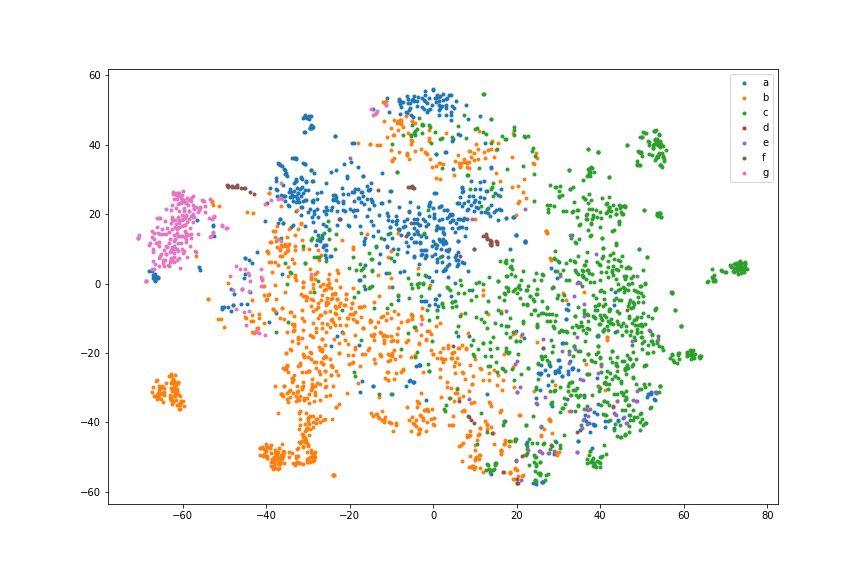
\includegraphics[width=0.49\linewidth]{latex/imgs/tsne_1_layer_with_schedule_1024_minloss.png}
  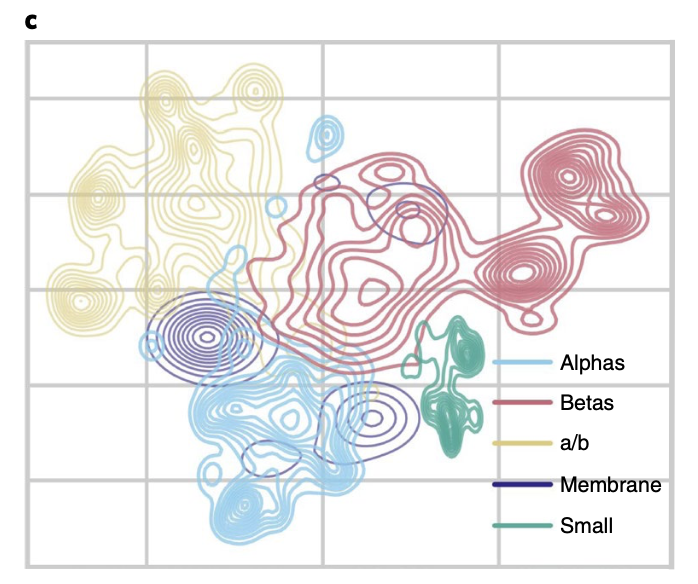
\includegraphics[width=0.49\linewidth]{latex/imgs/unirep_tsne.png}
  \caption{Left image is our best model's TSNE dimensionality reduction, the right image is an image taken from Unirep\cite{unirep}}
  \label{fig:unirep_comp}
\end{figure}